\lab{Applications}{Image Segmentation}{Image Segmentation}

\objective{Understand some basic applications of eigenvalues to graph theory.}
\label{lab:ImgSeg_eigenvalues}

\section*{Graph Theory}
\begin{figure}

 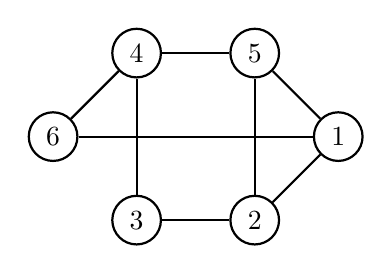
\begin{tikzpicture}[auto,node distance=1.5cm,
 thick,main node/.style={circle,draw}]

  \node[main node] (5) [] {6};
  \node[main node] (2) [below right of=5] {3};
  \node[main node] (3) [above right of=5] {4};
  \node[main node] (4) [right of=3] {5};
  \node[main node] (1) [right of=2] {2};
  \node[main node] (0) [below right of=4] {1};

  \foreach \s/\t in {5/3, 3/4, 4/0, 0/1, 1/2, 2/3, 1/4, 5/0} {
   \path[draw] (\s) edge (\t);}
\end{tikzpicture}
\caption{An undirected graph that is connected.}
\label{fig:example_graph}
\end{figure}

\begin{figure}

 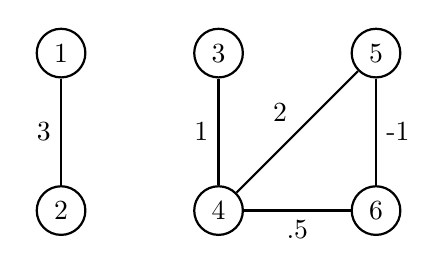
\begin{tikzpicture}[auto,node distance=2cm,
 thick,main node/.style={circle,draw}]

  \node[main node] (0) [] {1};
  \node[main node] (1) [below of=0] {2};
  \node[main node] (2) [right of=0] {3};
  \node[main node] (3) [below of=2] {4};
  \node[main node] (4) [right of=2] {5};
  \node[main node] (5) [right of=3] {6};

   \path[draw] (0) edge node [left] {3} (1);
   \path[draw] (2) edge node [left] {1} (3);
   \path[draw] (4) edge node{-1} (5);
   \path[draw] (3) edge node{2} (4);
   \path[draw] (3) edge node [below]{.5} (5);
\end{tikzpicture}
\caption{A weighted undirected graph that is not connected.}
\label{fig:example_graph2}
\end{figure}

% \begin{tikzpicture}[auto,node distance=1.5cm,
% thick,main node/.style={circle,draw}]
%
%  \node[main node] (2) [] {2};
%  \node[main node] (1) [below left of=2] {1};
%  \node[main node] (0) [below right of=2] {0};
%
%  \foreach \s/\t in {1/1, 1/2, 1/3, 2/3} {
%   \path[draw] (\s) edge (\t);}
%\end{tikzpicture}
%\caption{An undirected graph that is not simple.}
%\label{fig:example_graph}
%\end{figure}


%\begin{figure}
% \begin{tikzpicture}[->,>=stealth',shorten >=1pt,auto,node distance=1.5cm,
% thick,main node/.style={circle,draw}]
%
%  \node[main node] (A) [] {A};
%  \node[main node] (B) [below of=A] {B};
%  \node[main node] (C) [right of=A] {C};
%  \node[main node] (D) [below of=C] {D};
%  \node[main node] (E) [right of=C] {E};
%  \node[main node] (F) [right of=D] {F};
%
%  \foreach \s/\t in {A/C, B/A, B/D, C/E, C/F, D/C} {
%   \path[draw] (\s) edge (\t);}
%\end{tikzpicture}
%\caption{A simple directed graph}
%\end{figure}



Graphs represent relationships between objects.
%For example, the transition diagram in Figure \ref{fig:markov1} in Lab \ref{lab:EigSolve} shows the relationship between states in a Markov chain.
An \emph{undirected graph} is a set of nodes (or vertices) and edges, where each edge connects exactly two nodes and (see Figure \ref{fig:example_graph}).
A \emph{directed graph} has the additional information of an arrow on each edge. 
In this lab we will only consider undirected graphs, which we will simply call graphs (unless we wish to emphasize the fact that they are undirected).

%A graph is \emph{simple} if no edge connects a node to itself. 
%The graph in Figure [TODO!] is simple, but the graph in Figure [TODO!] is not.

A \emph{weighted} graph is a graph with a weight attached to each edge.
For example, a weighted graph could represent a collection of cities with roads connecting them.
The vertices would be cities, the edges roads, and weight of an edge would be the length of a road.
Such a graph is depicted as in Figure \ref{fig:example_graph2}.

Any graph can be thought of as a weighted graph by assigning a weight of 1 to each edge.

\subsection*{Adjacency, degree, and Laplacian matrices}
We will now introduce three special matrices associated to a graph. 
Throughout this section, assume we are working with a weighted undirected graph with $N$ nodes, and that $w_{ij}$ is the weight attached to the edge connecting node $i$ and node $j$.
We first define the adjacency matrix.

\begin{definition} The \emph{adjacency matrix} is an $N \times N$ matrix whose $(i,j)$-th entry is
\begin{center}
	$ \begin{cases}  w_{ij} & \mbox{if an edge connects node i and node j} \\ 0 & \mbox{otherwise.} \end{cases}$
\end{center}
% If the graph is not simple, there are differing conventions for how to define the diagonal of the adjacency matrix.
\end{definition}

For example, the graph in Figure \ref{fig:example_graph} has the adjacency matrix $A_1$ and the graph in Figure \ref{fig:example_graph2} has the adjacency matrix $A_2$, where
\[
A_1 = \begin{pmatrix}
0 & 1 & 0 & 0 & 1 & 1\\
1 & 0 & 1 & 0 & 1 & 0\\
0 & 1 & 0 & 1 & 0 & 0\\
0 & 0 & 1 & 0 & 1 & 1\\
1 & 1 & 0 & 1 & 0 & 0\\
1 & 0 & 0 & 1 & 0 & 0
\end{pmatrix}. \qquad A_2 = 
 \begin{pmatrix}
0 & 3 & 0 & 0 & 0 & 0\\
3 & 0 & 0 & 0 & 0 & 0\\
0 & 0 & 0 & 1 & 0 & 0\\
0 & 0 & 1 & 0 & 2 & .5\\
0 & 0 & 0 & 2 & 0 & -1\\
0 & 0 & 0 & .5 & -1 & 0
\end{pmatrix}
\]
Notice that these adjacency matrices are symmetric. This will always be the case for undirected graphs.

\begin{comment}
Raising the adjacency matrix to a power yields some very interesting information.
We can discover the number of paths of length $n$ between two nodes by raising a graph's adjacency matrix to the $n$th power.
For example, by squaring $A$, we can find the number of paths of length two between every pair of nodes.
\begin{lstlisting}
>>> A = np.array([[0,1,0,0,1,0],[1,0,1,0,1,0],
                  [0,1,0,1,0,0],[0,0,1,0,1,1],
                  [1,1,0,1,0,0],[0,0,0,1,0,0]])

>>> np.linalg.matrix_power(A,2)
array([[2, 1, 1, 1, 1, 0],
       [1, 3, 0, 2, 1, 0],
       [1, 0, 2, 0, 2, 1],
       [1, 2, 0, 3, 0, 0],
       [1, 1, 2, 0, 3, 1],
       [0, 0, 1, 0, 1, 1]])
\end{lstlisting}
We can see that no paths of length two exist between node 0 and node 5 because $A^2_{0,5} = 0$.
By calculating $A^6$ we can find the number of paths of length six from node 3 to itself.
\begin{lstlisting}
>>> np.linalg.matrix_power(A, 6)
array([[45, 54, 38, 45, 54, 16],
       [54, 86, 29, 77, 51, 11],
       [38, 29, 55, 15, 70, 27],
       [45, 77, 15, 75, 31,  4],
       [54, 51, 70, 31, 93, 34],
       [16, 11, 27,  4, 34, 14]])
\end{lstlisting}
We see that there are 75 unique paths of length six from node 3 to itself.
Imagine trying to count all of those paths by hand!
It would be very easy to count incorrectly.
This method makes it very simple to count paths without mistakes.

Adjacency matrices can also be composed of \li{True} and \li{False} values.
In this case, the $n$th power of such a matrix (using boolean arithmetic)
is again a matrix of
boolean values which simply indicate whether there exists a path of length $n$ between the given pair of nodes, rather than indicating the number of such
paths.

\begin{problem}
Let the following matrix represent a directed graph
\[
\begin{pmatrix}
0 & 0 & 1 & 0 & 1 & 0 & 1 \\
1 & 0 & 0 & 0 & 0 & 1 & 0 \\
0 & 0 & 0 & 0 & 0 & 1 & 0 \\
1 & 0 & 0 & 0 & 1 & 0 & 0 \\
0 & 0 & 0 & 1 & 0 & 0 & 0 \\
0 & 0 & 1 & 0 & 0 & 0 & 1 \\
0 & 1 & 0 & 0 & 0 & 0 & 0
\end{pmatrix}
\]
Between which pair of nodes does there exist the greatest number of paths
of length five?
From which node to which node is there no path of length seven?
\end{problem}
\end{comment}

The second matrix is the degree matrix. 
\begin{definition} The \emph{degree matrix} is an $N \times N$ diagonal matrix whose $(i,i)$-th entry is
\[ 
\sum_{j=1}^N w_{ij}.
\]
This quantity is just the sum of the weight of each edge that touches node $i$.
\end{definition}
%For a directed graph, each node has an \emph{out-degree} (the number of edges directed away from a node) and an \emph{in-degree} (the number edges directed toward a node).
We call the $(i, i)-th$ entry of the degree matrix the \emph{degree} of node $i$. As an example, the degree matrices of the graphs in Figures \ref{fig:example_graph} and \ref{fig:example_graph2} are $D_1$ and $D_2$, respectively, where

\[
D_1 = \begin{pmatrix}
3 & 0 & 0 & 0 & 0 & 0\\
0 & 3 & 0 & 0 & 0 & 0\\
0 & 0 & 2 & 0 & 0 & 0\\
0 & 0 & 0 & 3 & 0 & 0\\
0 & 0 & 0 & 0 & 3 & 0\\
0 & 0 & 0 & 0 & 0 & 2
\end{pmatrix}. \qquad D_2 = 
 \begin{pmatrix}
3 & 0 & 0 & 0 & 0 & 0\\
0 & 3 & 0 & 0 & 0 & 0\\
0 & 0 & 1 & 0 & 0 & 0\\
0 & 0 & 0 & 3.5 & 0 & 0\\
0 & 0 & 0 & 0 & 1 & 0\\
0 & 0 & 0 & 0 & 0 & -.5
\end{pmatrix}
\]

Finally, we can combine the degree matrix and the adjacency matrix into the Laplacian matrix.
% Wikipedia defines the Laplacian of a simple graph only. I don't know why.
% The graph in our application is NOT simple. 
% However, the non-simple parts cancel out, meaning that the Laplacian of the graph is the same as if you removed all self edges and then computed the Laplacian.
% So I just define the Laplacian this way and don't talk about simple graphs.
\begin{definition}
The \emph{Laplacian matrix} of a graph is 
\[D - A \]
where $D$ is the degree matrix and $A$ is the adjacency matrix of the graph.
\end{definition}

For example, the Laplacian matrix of the graphs in Figures \ref{fig:example_graph} and \ref{fig:example_graph2} are $L_1$ and $L_2$, respectively, where

\[
L_1 = \begin{pmatrix}
3 & -1 & 0 & 0 & -1 & -1\\
-1 & 3 & -1 & 0 & -1 & 0\\
0 & -1 & 2 & -1 & 0 & 0\\
0 & 0 & -1 & 3 & -1 & -1\\
-1 & -1 & 0 & -1 & 3& 0\\
-1 & 0 & 0 & -1 & 0 & 2
\end{pmatrix}. \qquad L_2 = 
 \begin{pmatrix}
3 & -3 & 0 & 0 & 0 & 0\\
-3 & 3 & 0 & 0 & 0 & 0\\
0 & 0 & 1 & -1 & 0 & 0\\
0 & 0 & -1 & 3.5 & -2 & -.5\\
0 & 0 & 0 & -2 & 1 & 1\\
0 & 0 & 0 &- .5 & 1 & -.5
\end{pmatrix}
\]


In this lab we will learn about graphs by studying their Laplacian matrices.
While the Laplacian matrix seems simple, we can learn surprising things from its eigenvalues.


\begin{problem}
Write a function that accepts the adjacency matrix of a graph as an argument. 
Your function should return the Laplacian matrix. 
Hint: You can compute the diagonal of the degree matrix in one line by summing over an axis (see Lab \ref{lab:NumPyArrays}).
Another hint: Test your function on the graphs in Figures \ref{fig:example_graph} and \ref{fig:example_graph2}.
\label{prob:laplacian}
\end{problem}



\subsection*{Connectivity: first application of Laplacians}

A \emph{connected graph} is a graph where every vertex is connected to every other vertex by at least one path.
The graph in Figure \ref{fig:example_graph} is connected, whereas the graph in Figure \ref{fig:example_graph2} is not.
In applications, it is often important to know if a graph is connected.
A naive approach to determine connectivity of a graph is to search every possible path from each vertex.
While this works for very small graphs, most interesting graphs will have thousands of vertices (for example, the internet), and for such graphs this approach is not feasible.

Fortunately, there is a better way.
Recall that the adjacency matrix of an undirected graph is always symmetric. 
Thus, it will have real eigenvalues. 
Surprisingly, a graph is connected if the second smallest eigenvalue of its Laplacian matrix is positive. [TODO: cite something!]
In many applications the Laplacian matrix is sparse, so by taking advantage of this sparsity, we can cheaply determine if a graph is connected.

\begin{problem}
\leavevmode
\begin{enumerate}
\item Write a function that accepts a symmetric adjacency matrix as an argument and returns the second smallest eigenvalue of the Laplacian matrix.
Use the \li{scipy.linalg} package to compute the eigenvalue.

\item Here is a function that creates a random symmetric matrix of Boolean values with sparsity determined by the input \li{c}.
\begin{lstlisting}
def sparse_generator(n, c):
    ''' Return a symmetric nxn matrix with sparsity determined by c.
    Inputs:
        n -- an integer
        c -- a decimal number in [0,1]. Larger values of c will produce
             matrices with more entries equal to zero.
    '''
    A = np.random.rand(n**2).reshape((n, n))
    A = ( A > c**(.5) )
    return A.T.dot(A)
\end{lstlisting}
\end{enumerate}

Run your function from part 1 of this problem on matrices created by \li{sparse_generator} with inputs $n = 10, 100$ and $c = .25, .5, .95$. 
What do you notice about the likelihood that a random graph is connected?
\end{problem}


\section*{Image Segmentation: second application of Laplacians}

\begin{figure}
    \centering
    \begin{subfigure}{0.31\textwidth}
        
\includegraphics[width=\textwidth]{RegMon.png}
    \end{subfigure}
   \hspace*{\fill}
    \begin{subfigure}{0.31\textwidth}
        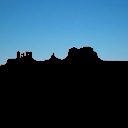
\includegraphics[width=\textwidth]{NegMon.png}
    \end{subfigure}
    \hspace*{\fill}
    \begin{subfigure}{0.31\textwidth}
        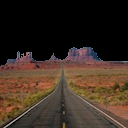
\includegraphics[width=\textwidth]{PosMon.png}
    \end{subfigure}
    
\caption{An image and its segments.}
\label{fig:monument}
\end{figure}
Image segmentation is the process of finding natural boundaries in an image (see for example Figure \ref{fig:monument}).
This is an easy task for humans, who can easily pick out portions of an image that ``belong together.''
In this lab, you will learn one way to program a computer to segment images.

The algorithm we will present comes from a paper by Jianbo Shi and Jitendra Malik in 2000 (\cite{Shi2000}).
Their idea is to represent an image as a weighted graph as follows. 
To a computer, an \emph{image} is a collection of \emph{pixels}. 
Each pixel has a brightness and coordinates describing its location in the image.
To define a graph representing this image, we let every pixel be a vertex.
Two pixels are connected if the distance between their coordinates is small (less than $r$).
The weight of the edge connecting two pixels is related their similarity in brightness, where a low weight means they are very different.

After defining this graph, we will segment the image by ``cutting'' (or removing) edges with low weights, which represent lines of high contrast in the image. 
The ``cut'' is the total weight of the edges removed. Thus, to segment an image, we wish to minimize the ``cut.''
We can ``cut'' an image multiple times to segment an image into more than two pieces.

Now let us define the adjacency matrix of the graph associated to an image. 
Since an $N \times N$ image has $N^2$ pixels, the adjacency matrix will be $N^2 \times N^2$.
After choosing a radius $r$ and some constants $\sigma_I$ and $\sigma_d$, we define the adjacency matrix to be $W = (w_{ij})$, where

\begin{equation}
\label{eq:adjacency}
w_{ij} = \begin{cases} \exp(-\frac{|I(i) - I(j)|}{\sigma_I^2}-\frac{d(i,j)}{\sigma_d^2}) & \mbox{ for $d(i,j) < r$} \\ 0 & \mbox{ otherwise,} \end{cases}
\end{equation}
where
\begin{itemize}
	\item$d(i,j)$ is the Euclidean distance between pixel $i$ and pixel $j$
	\item $|I(i) - I(j)|$ is the difference in brightness of pixels $i$ and $j$.
\end{itemize}

Notice that $W$ will be sparse as long as $r$ is small. Figure \ref{fig:adjacency} shows what the adjacency matrix looks like for a $4x4$ image when $r=1.2$.

\begin{figure}
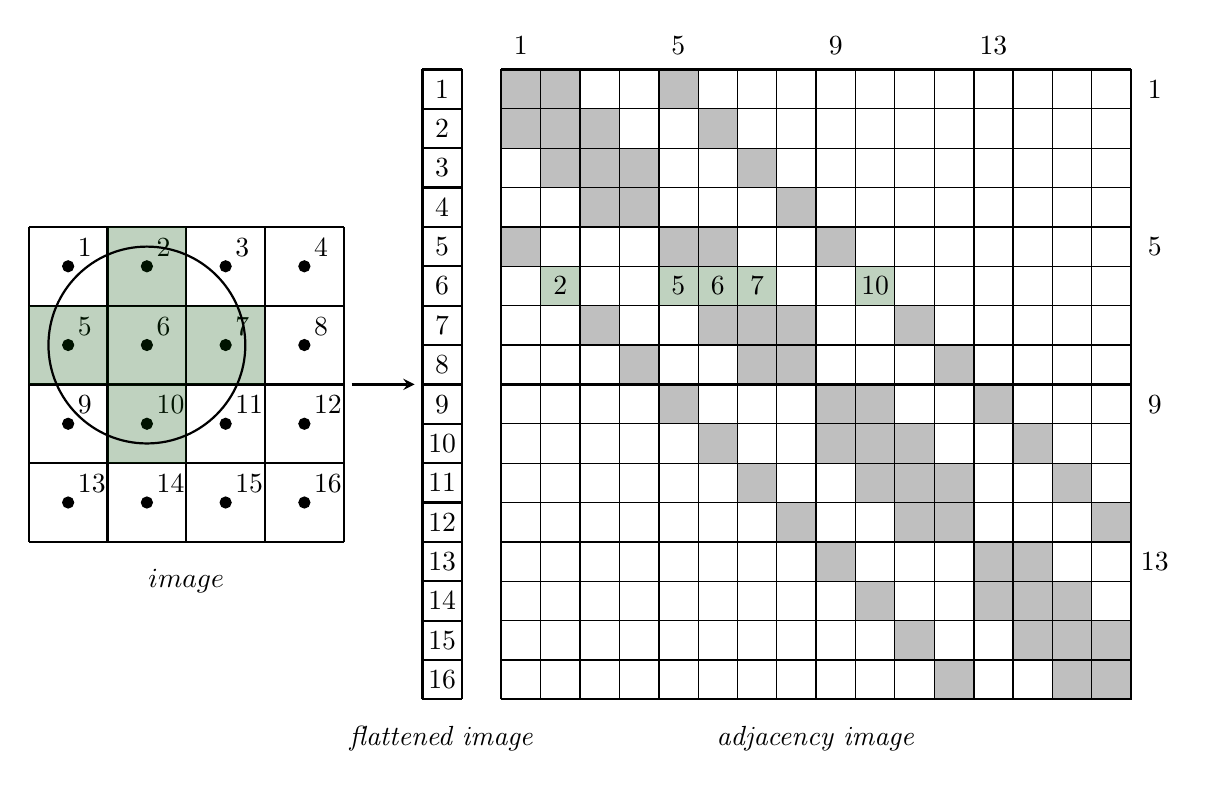
\begin{tikzpicture}[dot/.style={circle,fill=black,minimum 
	size=4pt,inner sep=0pt,outer sep=-1pt}, >=stealth]

%image
\draw[step=1,thick](2,0)grid(6,4);
%numbers 1-16
\foreach \x in {1,2,3,4}
	\foreach \y in {4}
		\node[draw=none, anchor=south west]at(\x+1.5, \y-.5){\x};
\foreach \x [evaluate=\x as \r using int(\x+4)]in {1,2,3,4}
	\foreach \y in {3}
		\node[draw=none, anchor=south west]at(\x+1.5, \y-.5){\r};
\foreach \x [evaluate=\x as \r using int(\x+8)] in {1,2,3,4}
	\foreach \y in {2}
		\node[draw=none, anchor=south west]at(\x+1.5, \y-.5){\r};
\foreach \x [evaluate=\x as \r using int(\x+12)] in {1,2,3,4}
	\foreach \y in {1}
		\node[draw=none, anchor=south west]at(\x+1.5, \y-.5){\r};

\node[draw=none](image)at(4, -.5){$image$};
\node[draw=none](flattened)at(7.25,-2.5){\textit{flattened image}};
\node[draw=none](adjacency)at(12,-2.5){\textit{adjacency image}};

%dots within grid
\foreach \x in {1,2,3,4}
	\foreach \y in {1,2,3,4}
		\node[draw, dot]at(\x+1.5,\y-.5){};

%color fill
\foreach \x/\y in {2/4, 1/3, 2/3, 3/3, 2/2} {\node[draw, minimum 
	size=1cm, fill=green!30!black, fill opacity=.25]at(\x+1.5,\y-.5){};}

%circle in image
\node[draw, circle, minimum size=2.5cm,thick](circle)at(3.5,2.5){};

%flattened image
\draw[step=.5, thick](6.999,-2)grid(7.5,6);
\foreach \x in {7}
	\foreach \y in {1,...,16}
		\node[draw=none]at(\x+.25,\y*-.5+6.25){\y};

\draw[->,thick](6.1, 2)--(6.9,2);

%adjancey matrix
\draw[step=.5](7.9999,-2)grid(16,6);
\draw[step=2,thick](7.999,-2)grid(16,6);

%outside labels
\foreach \x in {1,5,9,13} {\node[draw=none]at(\x*.5+7.75,6.3){\x};}
\foreach \y in {1,5,9,13}{\node[draw=none]at(16.3,\y*-.5+6.25){\y};}

%shading of boxes
\foreach \x/\y in {8.5/6, 9/6, 8.5/5.5, 9/5.5, 9.5/5.5,9/5,9.5/5,10/5, 
	9.5/4.5, 10/4.5, 10.5/6, 11/5.5,11.5/5, 12/4.5, 12.5/4, 
	13.5/3, 14/2.5, 14.5/2, 15/1.5, 15.5/1,16/.5, 10.5/4, 11/4, 11/3, 
	11.5/3,12/3, 11.5/2.5,12/2.5, 12.5/2, 13/2, 12.5/1.5, 13/1.5,
	13.5/1.5,13/1,13.5/1,14/1, 13.5/.5,14/.5, 14.5/0,15/0,14.5/-.5,
	15/-.5,15.5/-.5, 15/-1, 15.5/-1, 16/-1, 15.5/-1.5, 16/-1.5, 8.5/4,
	9.5/3,10/2.5,10.5/2,11/1.5,11.5/1,12/.5, 12.5/0, 13/-.5, 13.5/-1, 14/-1.5} 
	{\node[draw, minimum size=.5cm, fill=black, fill opacity=.25]
	at(\x-.25,\y-.25){};}

%green shaded boxes
\foreach \x/\y in {9/3.5,11/3.5, 11.5/3.5, 10.5/3.5, 13/3.5} {\node
	[draw, minimum size=.5cm, fill=green!30!black, fill opacity=.25]
	at(\x-.25,\y-.25){};}

\node[draw=none]at(8.75,3.25){2};
\node[draw=none]at(10.25,3.25){5};
\node[draw=none]at(10.75,3.25){6};
\node[draw=none]at(11.25,3.25){7};
\node[draw=none]at(12.75,3.25){10};

\end{tikzpicture}

\caption{The grid at left represents a $4\times4$ image, which has 16 pixels. Thus the adjacency matrix at right is $16 \times 16$. We have not calculated the weights in the adjacency matrix, but we have shaded the nonzero entries. For example, the $6^{th}$ row corresponds to the $6^{th}$ pixel. Within that row, entries are nonzero if they correspond to pixels that are at most 1.2 away from pixel 6.}
\label{fig:adjacency}
\end{figure}


\subsection*{Computing the adjacency matrix}
Let us write a function that accepts an image \li{img} and constants \li{radius}, \li{sigma_I}, and \li{sigma_d}. The function will return the adjacency matrix defined in (\ref{eq:adjacency}) and the diagonal of the corresponding degree matrix. The input \li{img} should be a 2-D array of brightness values. Here is the function definition, which includes some default values for the constants.
\begin{lstlisting}
1. def adjacency(img, radius=5.0, sigma_I = .15, sigma_d = 1.7):
\end{lstlisting}

Later, our function will iterate through the rows of the adjacency matrix, initializing one row at a time. Each row corresponds to a pixel of the original image. Thus, we begin by flattening the image (see Figure \ref{fig:adjacency}). We also store the dimensions of \li{img} for later.
\begin{lstlisting}
2.     flat_img = img.flatten()
3.     height, width = img.shape
\end{lstlisting}

Next we want to initialize the adjacency and degree matrices. As can be seen in Figure \ref{fig:adjacency}, the adjacency matrix should be sparse, so we initialize it as a sparse matrix \li{W}. The sparse matrix type \li{lil_matrix} is optimized for building a matrix one entry at a time, which is what we will do. On the other hand, we only need to compute the diagonal of the degree matrix, so we initialize this diagonal as a regular NumPy array \li{D}.
\begin{lstlisting}
4.     W = spar.lil_matrix((flat_img.size, flat_img.size), dtype=float)
5.     D = np.zeros((1, flat_img.size))
\end{lstlisting}

Now for each pixel in the image, we initialize the corresponding row of the adjacency matrix. 
The sum of the entries of this row will be the corresponding entry in \li{D}. 

The function \li{getNeighbors} returns two flat arrays: \li{indices} and \li{distances} (code is provided at the end of this lab). The array \li{indices} contains the indices of those pixels with \li{radius} of the input \li{pixel}. The array \li{distances} contains the corresponding distances of those pixels from the input \li{pixel} (all entries of \li{distances} will be at most \li{radius}). According to (\ref{eq:adjacency}), the array \li{indices} contains exactly the indices of the nonzero entries of the current row of \li{W}.\footnote{Note that \li{W} will be a symmetric matrix. We could possibly speed up this function a lot by taking advantage of this fact.}

\begin{lstlisting}
6.     for pixel in xrange(flat_img.size):
7.         indices, distances = getNeighbors(pixel, radius, height, width)
8.         weights = # weights[j] should be W[pixel, indices[j]]
9.         W[pixel, indices] = weights
10.        D[0,pixel] = weights.sum()
\end{lstlisting}

Finally, we convert \li{W} to the sparse matrix type \li{csc_matrix}, which is faster for computations. Then we return \li{W} and \li{D}. 
\begin{lstlisting}
11.    W = W.tocsc()
12.    return W, D
\end{lstlisting}


\begin{problem}
Finish writing the function \li{adjacency} described in this section by (a) adding comments and (b) filling in the following line.
\begin{lstlisting}
8.         weights = # weights[j] should be W[pixel, indices[j]]
\end{lstlisting}
Your computation should use (\ref{eq:adjacency}) and take exactly one line.

Images are typically stored as 2-D arrays of RGB values. To convert such an array to a 2-D array of brightness values, run the following code.
\begin{lstlisting}
# read in the image
img_color = plt.imread('dream.png')
# convert to grayscale
img = (img_color[:,:,0]+img_color[:,:,1]+img_color[:,:,2])/3.0
\end{lstlisting}
Test your function on the image \li{dream.png} (which is currently a 2-D array of RGB values).


%Notice that for each pixel you can save time by only checking the pixels $r$ rows and columns away.
%For that you'll have to handle the pixels on the edges and corners of the image carefully.
%I gave them new helper code, which abstracts away the edge cases.
\label{prob:adjacency_dream}
\end{problem}

\subsection*{Minimizing the 'cut'}

As was mentioned before, we are trying to minimize the `cut', or the total weight of the edges we remove to create segments. 
Let $L$ be the Laplacian of the adjacency matrix defined in \ref{eq:adjacency} and let $D$ be the degree matrix.
Shi and Malik proved that we can minimize the `cut' by finding the second smallest eigenvalue of $D^{-1/2}LD^{-1/2}$.
Because both $D$ and $L$ will be symmetric matrices, all eigenvalues of $D^{-1/2}LD^{-1/2}$ will be real, and so it makes sense to ask for the second smallest one.

The eigenvector associated to the second smallest eigenvalue will have $N^2$ entries, some positive and some negative. 
We can reshape this vector to be an $N \times N$ mask defining two segments, segments that correspond to the positive and negative values of the eigenvector.
Shi and Malik proved that these are the segments we desire. 

Here is the definition of a function that will segment an image.
\begin{lstlisting}
1. def segment(img):
\end{lstlisting}

We use the function \li{adjacency} from Problem \ref{prob:adjacency_dream} to compute the adjacency matrix and the diagonal of the degree matrices of the image. 
\begin{lstlisting}
2.     W, D = adjacency(img)
\end{lstlisting}

Next we create sparse matrices corresponding to $D$ and $D^{-1/2}$ in Shi and Malik's algorithm. Remember that the sparse matrix type \li{csc_matrix} is best for computations.
\begin{lstlisting}
3.     Dsq = # calculate the square root of D
4.     D_matrix = spar.spdiags(D, 0, D.shape[1], D.shape[1], format = 'csc')
5.     Dsq_matrix = # create a sparse matrix with diagonal Dsq
\end{lstlisting}
Now it is simple to compute $D^{-1/2}LD^{-1/2}$. We call this matrix \li{P}.
\begin{lstlisting}
6.     L = # compute the Laplacian
7.     P = # compute D^{-1/2}*L*D^{-1/2} as in Shi and Malik's algorithm
\end{lstlisting}
According to Shi and Malik, we need the eigenvector corresponding to the second smallest eigenvalue of \li{P}. We compute this with the \li{eigs()} method of the \li{scipy.sparse.linalg} module. We set the parameter \li{which='SR'} in the function call in order to compute the eigenvalues with Smallest Real part and their corresponding eigenvectors. The parameter \li{k} in the function call can be used to specify how many eigenvalues the method computes.
\begin{lstlisting}
8.     e = # compute the two smallest eigenvalues of P and their eigenvectors
9.     eigvec = # eigenvector of the second smallest eigenvalue
\end{lstlisting}

Next we create a mask that is \li{True} wherever \li{eigvec} is positive and reshape it to be the size of \li{img}. 
\begin{lstlisting}
10.    mask = # create mask
\end{lstlisting}
Once we have a mask of True-False values, we multiply it by the image entrywise. This zeros out the pixels in the matrix corresponding to the \li{False} entries in the mask and leaves the pixels corresponding to \li{True} entries unaffected. We can negate the mask using the tilde operator, which lets us compute the other segment of the image. Finally we return the two segments.
\begin{lstlisting}
11.    pos = # compute positive segment
12.    neg = # compute negative segment
13.    return pos, neg
\end{lstlisting}



\begin{problem} Finish writing the function \li{segment} described in this section by (a) adding comments and (b) filling in the missing lines. 
You should be able to fill in these lines with exactly the space indicated. Test your function on the image \li{dream.png}. Your segments should look like the segments in Figure \ref{fig:dream_solution} (the original image is on the left). Here are some hints:

\begin{enumerate}
\item Note that in Line 6, you should NOT use your solution to Problem \ref{prob:laplacian}, because in this problem we are working with sparse matrices, and you have already computed the degree matrix.

\item Also, in Line 7, multiply sparse matrices \li{A} and \li{B} with \li{A.dot(B)}.
\item Here is some code that will plot the segments \li{neg} and \li{pos} as well as the original \li{img}.
\begin{lstlisting}
plt.subplot(131)
plt.imshow(neg)
plt.subplot(132)
plt.imshow(pos)
plt.subplot(133)
plt.imshow(img_color)
plt.show()
\end{lstlisting}

\end{enumerate}

\end{problem}

\begin{figure}
\centering
    \centering
    \begin{subfigure}{0.31\textwidth}
        
\includegraphics[width=\textwidth]{RegDream.png}
    \end{subfigure}
    \hspace*{\fill}
    \begin{subfigure}{0.31\textwidth}
        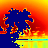
\includegraphics[width=\textwidth]{NegDream.png}
    \end{subfigure}
    \hspace*{\fill}
    \begin{subfigure}{0.31\textwidth}
        
\includegraphics[width=\textwidth]{PosDream.png}
    \end{subfigure}
\caption{Segments of \li{dream.png}}
\label{fig:dream_solution}
\end{figure}

\section*{Appendix: helper code for Problem \ref{prob:adjacency_dream}}
Here is the function \li{getNeighbors} which you can use to compute the adjacency matrix of an image, as in Problem \ref{prob:adjacency_dream}.

\lstinputlisting[style=fromfile]{getNeighbors.py}